\section{Ortopædkirurgisk afdeling på Aalborg Universitetshospital}
OA behandler primært skader på bevægeapparatet, herunder knogler, muskler, sener og led. Afdelingen er opdelt i $10$ fagområder: børneortopædkirurgi, knogle- og rekonstruktion, fod- og ankelkirurgi, knæ- og hoftekirurgi, håndkirurgi, ryg- og bækkenkirurgi, knæ- og idrætsskader, tumor- og sarkomkirurgi, amputationer og sår samt traumatologi. Afdelingen er yderligere opdelt i fem afsnit, herunder sengeafsnit O$1$ samt O$2$, operationsafsnit, sammedagskirurgisk afsnit O$6$ samt ambulatorium. 
Sengeafsnit O$1$ behandler bl.a. brud og skader på hånden, lårbenshalsen samt sportskader i knæet. Derudover behandles forbrændinger og ætsninger. Sengeafsnit O$2$ varetager børneoperationer, ryglidelser, fod- og ankelskader samt bækkenbrud og patienter med mange brud. Operationsafsnittet udfører de længerevarende operationer samt de operationer, der kræver speciallægeviden. Sammedagskirurgisk afsnit O$6$ foretager de mindre operative indgreb. Det sidste afsnit, ambulatorium, kontrollerer patienter, der har behov for kontrol før eller efter en operation.\cite{Aalborg2016}

\subsection{Personalets arbejdsgang} \label{arb_per}
På OA arbejder personalet i gennemsnit $37$ timer om ugen over en periode på otte uger\cite{Danske2015}[\ref{bilagO1},\ref{bilagO2}]. Vagterne består både af dag- og nattevagter. Over en arbejdsdag er der indlagt tre vagtskifte, hvor det nye vagthold har et kvarter til at sætte sig ind i, hvilke arbejdsopgaver samt patienter de skal varetage. Der er indlagt betalte pauser i personalets arbejdsdag, hvilket betyder, at personalet skal være til rådighed under pausen. Sygeplejersker arbejder ofte i par, hvor de sammen varetager to til otte patienter om dagen, mens de ofte varetager flere patienter på aftenvagter.[\ref{bilagO1}]

\subsection{Patienter}
OA modtager både elektive samt akutte patienter. Elektive patienter omfatter både indlagte og ambulante patienter. Ved pludselig forværret tilstand kan elektive patienter skifte status fra elektiv til akut. Akutte patienter defineres som personer, der er henvist til hospitalet efter en akut opstået tilstand.\cite{RegionNord2016} En fordeling af de elektive og akutte patienter fremgår af \figref{elektivvsakut}.

\begin{figure}[H]
	\flushleft 
	\centering
	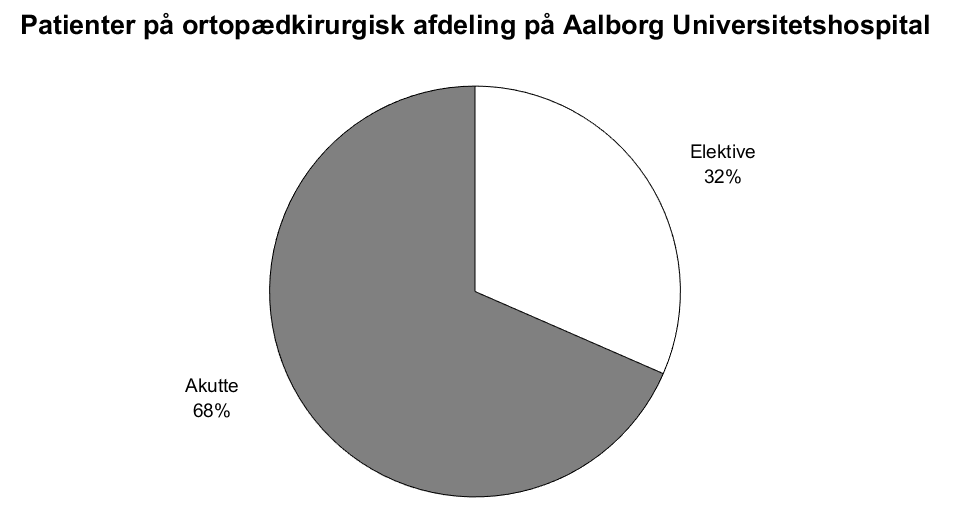
\includegraphics[scale=0.55]{figures/elektivvsakut.png}
	\flushleft
	\caption{\textit{Fordeling af elektive og akutte patienter på OA målt over en periode fra juli til og med oktober år $2014$.}\cite{REOS}}
	\label{elektivvsakut}
	\end{figure}

\noindent
Af \figref{elektivvsakut} illustreres det, at fordelingen mellem elektive og akutte patienter ikke er ligeligt fordelt på OA. Der ses over en periode i år $2014$, at de elektive patienter udgør $32~\%$ og de akutte udgør $68~\%$ af afdelingens patienter \\

\subsection{Planlægning af patienter} \label{book}
På OA er lægesekretæren ansvarlig for indkaldelser samt planlægning af de elektive patienter. Planlægningen af de elektive patienter foregår med forbehold for akutte patienter. Dette betyder, at antallet af sengepladser ikke altid udnyttes fuldt ud. Operationsdatoen planlægges ofte ud fra patienternes eget ønske. Det kan være et ønske om en bestemt kirurg, tidsperiode eller blot den første ledige tid.[\ref{bilagsek}]

\noindent
De elektive patienter indlæggelses typisk mellem kl $7$ og $18$, hvorimod de akutte patienter indlæggelses på hele døgnet. Udskrivelsestidspunktet for elektive ses typisk mellem kl. $9$ og $18$, mens akutte typisk udskrives mellem kl. $8$ og $18$. Indlæggelses- og udskrivelsestidspunktet for akutte og elektive patienter i perioden fra juli til og med oktober år $2014$ fremgår af \figref{indlaegudskriv}.\cite{REOS}

\begin{figure}[H]
	%\flushleft 
	\centering
	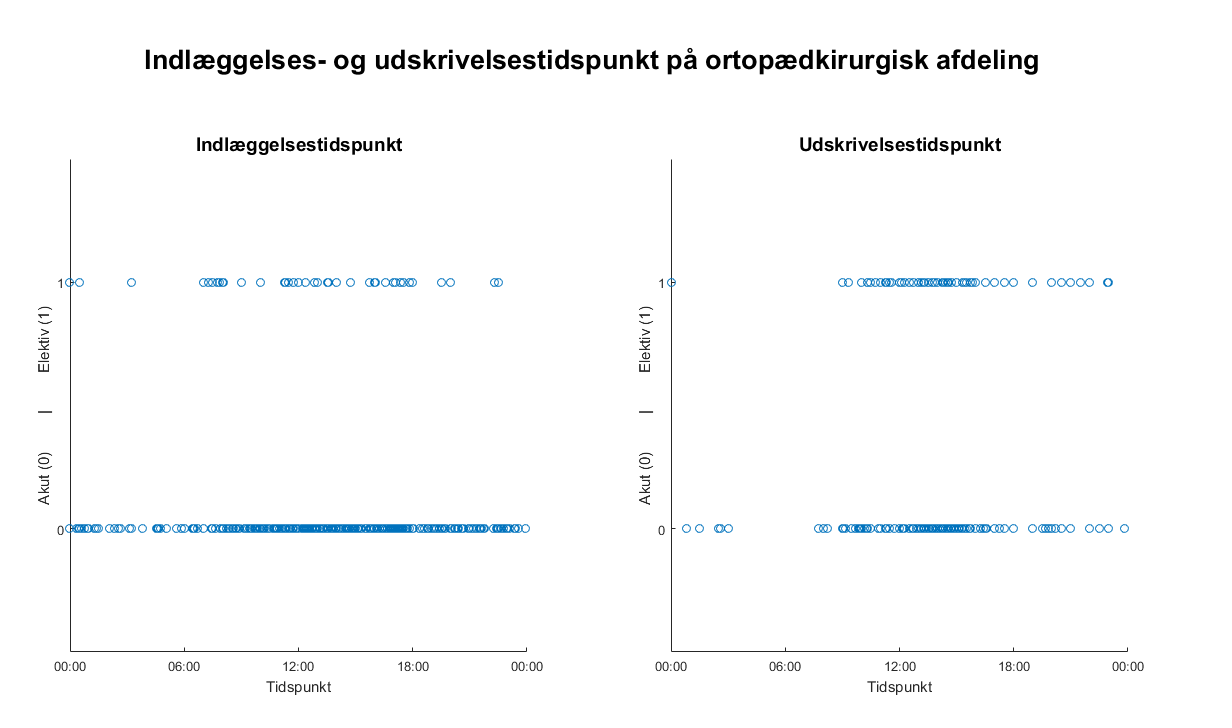
\includegraphics[scale=0.35]{figures/indlaegudskriv.png}
	%\flushleft
	\caption{\textit{Indlæggelses- og udskrivelsestidspunkt for akutte og elektive patienter over en periode fra juli til og med oktober år $2014$.}\cite{REOS}}
	\label{indlaegudskriv}
	\end{figure}
	
\noindent
Dette indikerer, at der er en grænse for, hvornår patienter udskrives. Patienter kan ikke udskrives uden lægens sammenstykke, hvorfor patienter generelt ikke udskrives mellem kl. $18$ og kl. $8$, på trods af, at de er udskrivningsparate. Lægens sammenstykke kan både fås ved tilseelse af patienter samt pr. telefon. Patienter, der har behov for hjemmepleje kan ikke udskrives før kommunen er kontaktet, dette skal forekomme før kl. $12$ på den pågældende dag patienten skal udskrives.[\ref{bilagO2}]

